\hypertarget{krediet-en-bankieren}{%
\chapter{Krediet en Bankieren}\label{krediet-en-bankieren}}

\begin{blockquotebox}
    Alle vormen van menselijke organisatie zijn op een bepaalde manier gekoppeld aan geldtransacties. Wanneer je dus het geldsysteem van een land of zelfs van de hele wereld vernietigt, maak je veel meer dan alleen een enkel facet kapot; je ontwricht in feite de fundamenten van alle menselijke interacties. Als je het monetaire systeem vernietigt, maak je de basis van alle menselijke relaties kapot. Wanneer we het over geld hebben, dan hebben we het over een thema waarbij overheden het uiterste hebben gedaan wat denkbaar is: de markt vernietigen, het ondermijnen van menselijke samenwerking en het vernietigen van alle vormen van vreedzaam menselijk contact.
    \par\raggedleft--- Ludwig von Mises\index{Ludwig von Mises}
\end{blockquotebox}
\footautocite{155}

\hypertarget{bankieren}{%
\section{Bankieren}\label{bankieren}}

Naarmate de tijdsvoorkeur\index{tijdsvoorkeur} afneemt, sparen individuen meer, waardoor ze als gevolg ook meer gaan investeren, wat leidt tot een stijging van de productiviteit en op zijn beurt de hoeveelheid spaargeld die voor hen beschikbaar is. Wanneer de hoeveelheid spaargeld groeit en de arbeidsdeling\index{arbeidsdeling} complexer wordt, ontwikkelt het beheer van geld zich tot een dienst die op de markt wordt aangeboden door gespecialiseerde professionals. De ontwikkeling van de arbeidsdeling\index{arbeidsdeling} leidt tot meer specialisatie in alle goederen en diensten, en voor geld is dat niet anders. Net als bij voedsel, kleding of huizen, verhoogt specialisatie de productiviteit waarmee een goed op de markt wordt aangeboden. Het bankwezen is de sector die zich heeft gespecialiseerd in het beheer van geld en heeft twee essentiële functies: het beheren van deposito\textquotesingle s en investeringen.

Op individueel niveau kunnen we zien hoe een lagere tijdsvoorkeur\index{tijdsvoorkeur} leidt tot uitgestelde voldoening en meer spaargeld, investeringen, productiviteit en economische overvloed. Op het niveau van de markteconomie, waarbij er sprake is van arbeidsdeling\index{arbeidsdeling} op grote onpersoonlijke schaal en het gebruik van geld als gemeenschappelijk ruil\index{ruil}- en spaarmiddel\index{spaarmiddel}, verhoogt het bankieren de productiviteit van sparen en investeren, waardoor een grotere kapitaalaccumulatie en een hogere productiviteit mogelijk worden. Iedereen in de maatschappij heeft er baat bij dat anderen op deze manier hun tijdsvoorkeur\index{tijdsvoorkeur} verlagen. Met andere woorden, andermans spaargeld verhoogt de productiviteit van jouw arbeid.

De primaire functie van bankieren is om spaarders te helpen om hun opgebouwde rijkdom te behouden en te beschermen tegen diefstal en verlies. Huizen zijn geoptimaliseerd wat betreft hun locatie, comfort en verschillende andere kenmerken, maar ze zijn niet optimaal beschermd voor diefstal. Een steeds meer gespecialiseerde economie zal voor individuen en bedrijven de mogelijkheid ontwikkelen om hun bezittingen te bewaren op plekken die gespecialiseerd zijn voor het veilig bewaren van deze bezittingen. Banken zullen deposito\textquotesingle s accepteren en hun eigenaren laten betalen voor het gebruik van deze diensten. Door een faciliteit te bouwen die gespecialiseerd is in het veiligstellen van spaartegoeden\index{spaartegoeden}, kan het gebouw worden geoptimaliseerd voor veiligheid en beveiliging tegen diefstal. Door een kleine vergoeding in rekening te brengen aan veel vermogende individuen, kunnen bankiers de bouw en exploitatie van veilige faciliteiten financieren die minder snel beroofd zullen worden dan individuele huizen of werkplekken. Depositobankieren is in de basis, als het veilig, verstandig en eerlijk gebeurt, een saaie en grotendeels oninteressante dienst die niet veel economische analyse verdient. De interessante en tragische gevolgen ontvouwen zich pas op het moment dat depositobankieren wordt misbruikt. Helaas voor spaarders wordt depositobankieren zo vaak misbruikt dat veilig en saai bankieren tot het verleden behoort.

\hypertarget{krediet}{%
\section{Krediet}\label{krediet}}

De eerste functie van bankieren is het aanhouden van spaartegoeden\index{spaartegoeden} namens hun eigenaars. De tweede rol is het investeren van dit spaargeld om winsten te realiseren die het spaargeld doen toenemen, terwijl men het risico\index{risico} neemt om het te verliezen. Het verstrekken van krediet\index{krediet} stelt de spaarder in staat zijn spaargeld te laten renderen. Het krediet\index{krediet} zal ingezet worden ten dienste van een ondernemer wiens bedrijf\index{bedrijf} zich bezighoudt met economische productie\index{productie}. Door niet te consumeren en geen geld op te potten, wordt de spaarder een investeerder en stelt zij haar spaargeld ter beschikking om inputs voor een productieproces\index{productieproces} te kopen. De productiefactoren worden vervolgens gecombineerd om de output te produceren die op de markt wordt verkocht, idealiter tegen een opbrengst die hoger is dan de kosten, waardoor de ondernemer en de kapitalisten worden beloond met winst. Als het bedrijf\index{bedrijf} geen winst maakt, zijn de investeerders hun spaargeld kwijt.

Terwijl een kapitalist haar eigen geld uitleent aan een ondernemer, leent een bank\index{bank} het geld van spaarders uit. Ze specialiseert zich in de toewijzing van investeringen, terwijl ze de spaarders laat specialiseren in datgene waarmee ze hun inkomen verdienen. De introductie van specialisatie en arbeidsdeling\index{arbeidsdeling} in kapitaalinvesteringen zorgt ervoor dat de productiviteit toeneemt. Het stelt individuen in staat om geld te investeren waarvoor ze geen voor de hand liggend nut hebben in hun eigen werk. Investeren is dus niet langer afhankelijk van het vermogen van een bedrijf\index{bedrijf} zelf om te groeien. Door te investeren in productielijnen die niet direct gerelateerd zijn aan de eigen sector, kunnen investeerders zich indekken tegen het falen van hun bedrijf\index{bedrijf} of tegen verstoringen in hun branche.

De taak van bankiers is om op te treden als tussenpersoon tussen de spaarder en de ondernemer. Ze voeren een risico\index{risico}-analyse uit op een groot aantal potentiële investeringen en geven op basis daarvan een deskundig oordeel over welke projecten het waard zijn om te financieren met het spaargeld van de spaarders. Dankzij de functie van een investeringsbankier kunnen spaarders de selectie van investeringen delegeren aan professionals, en kunnen ondernemers het benodigde kapitaal\index{kapitaal} bij de bank\index{bank} halen in plaats van te proberen het bij ongespecialiseerde individuen op te halen.

Echter is niet al het bankkrediet hetzelfde. Mises maakt een belangrijk onderscheid tussen twee verschillende soorten bankkrediet: goederenkrediet en circulatiekrediet.\autocite{156} De rest van dit hoofdstuk gaat over goederenkrediet, terwijl het volgende hoofdstuk over circulatiekrediet gaat.

\hypertarget{goederenkrediet}{%
\section{Goederenkrediet}\label{goederenkrediet}}

Mises gebruikt de term goederenkrediet om te verwijzen naar het krediet\index{krediet} dat geleend wordt door banken en verstrekt wordt aan ondernemers, waardoor banken louter tussenpersonen zijn die profiteren van het verschil tussen de rente\index{rente} die ze hun kredietgevers betalen en de rente\index{rente} die ze hun kredietnemers aanrekenen. Dit verschil komt voort uit de verwachting dat de specialisatie van de bank\index{bank} een hoger rendement oplevert dan wanneer een kredietverstrekker zelfstandig een tegenpartij probeert te vinden. Mises stelt dat een bank\index{bank}, in haar rol als verlener van goederenkrediet, de zogenaamde \textquotesingle gouden regel\textquotesingle{} moet handhaven. Deze regel luidt als volgt: ``Het krediet\index{krediet} dat een bank\index{bank} verschaft, moet zowel kwantitatief als kwalitatief overeenkomen met het krediet\index{krediet} dat zij heeft verkregen.'' Dit houdt in dat ``de datum waarop de verplichtingen van de bank\index{bank} opeisbaar worden, niet vooraf mag gaan aan de datum waarop haar overeenkomstige vorderingen kunnen worden geïnd.''\autocite{157} Met andere woorden, het is essentieel dat de hoeveelheid krediet\index{krediet} die de bank\index{bank} verstrekt niet groter is dan de hoeveelheid spaargeld die spaarders aan de bank\index{bank} hebben uitgeleend. Verder mag de datum waarop een bepaalde lening\index{lening} moet worden terugbetaald aan de bank\index{bank} niet later zijn dan de einddatum van de termijn waarvoor het krediet\index{krediet} door spaarders aan de bank\index{bank} werd aangeboden. Volgens de gouden regel kan de bank\index{bank} een deposito van een spaarder van één jaar niet voor twee jaar aan een ondernemer uitlenen, in de hoop dat in een jaar een andere kredietverstrekker wordt gevonden die een even groot deposito inlegt, waarmee de spaarder terugbetaald kan worden.

Wanneer er een discrepantie bestaat tussen de hoeveelheid krediet\index{krediet} die een bank\index{bank} opneemt en de hoeveelheid die zij uitleent, of wanneer er verschillen zijn in de looptijden, dan is de bank\index{bank} niet langer actief in het verstrekken van goederenkrediet maar in het creëren van circulatiekrediet. In zo'n geval draagt de bank\index{bank} niet simpelweg het geld van spaarders over aan ondernemers; ze creëert krediet\index{krediet} dat als geld fungeert, waardoor de totale geldhoeveelheid toeneemt. Dit heeft aanzienlijke gevolgen, die in het volgende hoofdstuk verder worden uitgewerkt.

Het onderscheidende kenmerk van goederenkrediet is dat het een offer vereist van de kredietgever. Om de lening te kunnen verstrekken moet iemand gedurende de hele looptijd afzien van toegang tot monetaire middelen ter waarde van het volledige leenbedrag. De kredietverstrekker ziet af van het geld in het heden met de verwachting in de toekomst een grotere uitbetaling te ontvangen. De lener krijgt daarentegen direct toegang tot het geld, maar betaalt extra kosten bij het terugbetalen van de lening\index{lening}. De rentevoet van de lening\index{lening} weerspiegelt de verschillen in waardering van tijd door beide partijen. De kredietverstrekker heeft een lagere tijdsvoorkeur\index{tijdsvoorkeur}, waardoor de waarde van de lening\index{lening} en de rente\index{rente} in de toekomst voor haar hoger is dan de hoofdsom, waardoor lenen tegen dat tarief voordelig is. De lener op zijn beurt heeft een hogere tijdsvoorkeur\index{tijdsvoorkeur}, waardoor de hoofdsom en de rente\index{rente} in de toekomst voor hem minder waard zijn dan de hoofdsom vandaag. Het verschil in tijdsvoorkeur\index{tijdsvoorkeur} tussen de twee maakt het voor hen mogelijk om een transactie aan te gaan.

\hypertarget{rentevoeten}{%
\section{Rentevoeten}\label{rentevoeten}}

In de traditionele economie worden rentetarieven gezien als de bepalende factor voor de hoeveelheid spaargeld in de markt, omdat individuen hun tijdsvoorkeur\index{tijdsvoorkeur} vergelijken met rentetarieven en dan beslissen of ze zullen sparen of niet. Dit is echter alleen houdbaar in een centraal geplande economie waar de rente\index{rente} door de overheid\index{overheid} wordt bepaald. Maar wat zou in een vrije markt de rente\index{rente} bepalen? Die wordt bepaald door de tijdsvoorkeur\index{tijdsvoorkeur} van mensen. Het kan niet bepaald worden door de productiviteit van de gefinancierde projecten omdat er projecten zijn op alle productiviteitsniveaus. De beschikbaarheid van kapitaal\index{kapitaal}, wat een functie is van tijdsvoorkeur\index{tijdsvoorkeur}, bepaalt welke projecten gefinancierd worden en welke niet, niet hun productiviteit. Tijdsvoorkeur zorgt ervoor dat het kapitaal\index{kapitaal} beschikbaar is, en de ondernemer probeert het toe te wijzen aan de projecten met het hoogst verwachte rendement.

\begin{blockquotebox}
De rol van de kapitalisten is dus een functie van de tijd, en hun inkomen vertegenwoordigt nauwkeurig het verschil in waarde tussen de huidige en toekomstige goederen. \textbf{Dit inkomen uit rente\index{rente} komt dus niet voort uit de concrete, heterogene kapitaalgoederen\index{kapitaalgoederen}, maar uit de tijdsinvestering.} Het ontstaat uit de bereidheid om huidige goederen op te offeren voor de aankoop van toekomstige goederen (de diensten van productiefactoren). Als gevolg van de aankopen krijgen de eigenaren van factoren hun geld in het heden voor een product dat pas in de toekomst zijn vruchten afwerpt.\footnotemark
\end{blockquotebox}
\footautocite{158}

De verhouding tussen de waarde die wordt toegekend aan een huidig goed en aan een identiek toekomstig goed wordt de natuurlijke rente\index{rente} (of evenwichtsrente) genoemd. De natuurlijke rente\index{rente} vertegenwoordigt het percentage dat wordt gerekend bovenop de waardering van een goed zodat een individu bereid is het goed in de toekomst te ontvangen. Iemand die bijvoorbeeld verwacht vandaag een zending van 10 kilogram maïs te ontvangen, zal een bepaalde premie wensen te ontvangen om de levering een jaar uit te stellen. De procentuele toename van de hoeveelheid die aan die persoon moet worden aangeboden om zijn consumptie\index{consumptie} uit te stellen, is de natuurlijke rentevoet.

Vanuit het perspectief van de Oostenrijkse School\index{Oostenrijkse School} hebben alle economische fenomenen hun oorsprong in menselijk handelen\index{menselijk handelen}, en dat is voor rente\index{rente} niet anders. Tijdsvoorkeur creëert het fenomeen van de natuurlijke rente\index{rente}. De tijdsvoorkeur\index{tijdsvoorkeur} die inherent is aan mensen, wordt onvermijdelijk weerspiegeld in een premie op huidige goederen voor toekomstige goederen; dit wordt op zijn beurt weerspiegeld in de markt voor geld, wat een marktgoed is dat niet verschilt van alle andere. Ervan uitgaande dat de waarde van de valuta constant blijft, zal iemand die vandaag een betaling van €100 tegoed heeft, een premie willen krijgen om de betaling een jaar uit te stellen, net zoals dat iemand een premie zou willen krijgen voor de 10 kilogram maïs. De aanwezigheid van de tijdsvoorkeur\index{tijdsvoorkeur} zelf is de bepalende factor en de oorsprong van natuurlijke rente\index{rente}.

De aanwezigheid van geld maakt het mogelijk om de natuurlijke rente\index{rente} te harmoniseren tussen goederen en individuen. Dit gebeurt door het ontstaan van een kredietmarkt waarin toekomstige geldverplichtingen worden verhandeld voor onmiddellijke betalingen, waardoor een algemeen geldende disconteringsvoet van de toekomst, oftewel een rentevoet, wordt vastgesteld. Met ``disconteren''\footnote{Noot van de vertalers. In dat geval wordt met “disconteren” het `afwaarderen van de toekomst' bedoeld, ofwel het omrekenen van toekomstige waarde naar huidige waarde. De disconteringsvoet is dus de mate waarop een individu de toekomst minder waardeert dan het heden.} wordt het minder waarderen van de toekomst bedoeld. De disconteringsvoet is dus de mate waarop een individu de toekomst minder waardeert dan het heden. Afwijkingen tussen de disconteringsvoet voor bepaalde goederen en de gangbare marktrente voor geld zullen mogelijkheden creëren voor winstgevende arbitrage in deze goederen, waardoor de rente\index{rente} op alle goederen binnen een smalle bandbreedte komt, die op de markt tot uiting komt als de marktrente. Hoppe beschrijft deze door de markt bepaalde rentevoet als ``de totale som van alle individuele tijdsvoorkeuren, die de maatschappelijke tijdsvoorkeur\index{tijdsvoorkeur} weerspiegelen, en die de maatschappelijke spaarmiddelen\index{spaarmiddelen} (ofwel het aanbod van huidige goederen die in ruil\index{ruil} worden aangeboden tegen toekomstige goederen) en de maatschappelijke investeringen (ofwel de vraag naar huidige goederen waarvan gedacht wordt dat ze toekomstige opbrengsten kunnen opleveren) in evenwicht brengen.''\autocite{159}

Hoewel individuele kapitaalgoederen\index{kapitaalgoederen} hun eigen markten\index{markten} hebben waarop ze worden verhandeld, wordt kapitaal\index{kapitaal} in een moderne monetaire economie verhandeld als een abstract goed door het lenen en investeren van geldbedragen. Spaargelden van de maatschappij worden beschikbaar gesteld aan financiële instellingen die ze uitlenen aan ondernemers die ze daarna gebruiken om er kapitaalgoederen\index{kapitaalgoederen} van te kopen. De vraag naar investeringen en de aankoop van kapitaalgoederen\index{kapitaalgoederen} is praktisch oneindig, omdat het bedenken van nieuwe ideeën door ondernemers veel gemakkelijker en goedkoper is dan het uitstellen van de consumptie\index{consumptie} van de huidige middelen. De beperkende factor voor de hoeveelheid investeringen is de hoeveelheid gespaard geld, en die wordt op zijn beurt beperkt door het verlangen en de noodzaak om te consumeren doordat tijdsvoorkeur\index{tijdsvoorkeur} altijd positief is. Het bestaan van kapitaalgoederen\index{kapitaalgoederen}, en kapitaalmarkten in het algemeen, is volledig afhankelijk van individuen die hun tijdsvoorkeur\index{tijdsvoorkeur} voldoende verlagen om het benodigde kapitaal\index{kapitaal} ter beschikking te stellen. Er is altijd vraag naar belegbaar geld en omdat er projecten zijn met een zeer breed scala aan rendementen, is het niet het verwachte rendement dat de rente\index{rente} bepaalt. Tijdsvoorkeur bepaalt de hoeveelheid middelen die uitgeleend kan worden, die vervolgens naar de projecten met de hoogste verwachte rendementen zullen gaan, waarvoor de leners bereid zijn de hoogste rente\index{rente} te betalen. Hoe meer er gespaard wordt, hoe lager de rente\index{rente}, hoe meer projecten er gefinancierd kunnen worden en hoe lager verwachte  rendement op het marginale project. Meer sparen leidt ook tot een groeiende diversiteit aan financieringsmechanismen, waardoor de liquiditeit\index{liquiditeit} van de kapitaalmarkt en de keuzemogelijkheden toenemen.

Door consumptie\index{consumptie} uit te stellen met als doel om investeerders van kapitaal\index{kapitaal} te voorzien, betaalt de kapitalist met zijn tijd. De kapitalist investeert zijn tijd in de onderneming door huidige goederen op te offeren voor goederen in de toekomst. Dit offer zorgt ervoor dat de arbeiders en de leveranciers van inputgoederen voor het productieproces\index{productieproces} betaald worden voordat de productie\index{productie} is afgerond en het eindproduct op de markt kan worden verkocht. Net zoals een afgezonderde visser tijd moet opofferen voor het vangen van vis om in plaats daarvan een hengel te kunnen bouwen, moet iemand de consumptie\index{consumptie} van middelen uitstellen om een productieproces\index{productieproces} te kunnen laten plaatsvinden. De ondernemer gebruikt de middelen en opofferingen van de kapitalist om de arbeiders, landeigenaren en verkopers van kapitaalgoederen\index{kapitaalgoederen} te betalen. Het productieproces\index{productieproces} neemt een bepaalde hoeveelheid tijd in beslag, waarna de ondernemer de eindproducten kan verkopen. Pas dan krijgt de kapitalist de afgesproken rente\index{rente} betaald. De arbeiders en de verkopers van inputgoederen worden echter betaald zodra ze de dienst verlenen, niet wanneer het product wordt verkocht, omdat ze hun tijd niet in de onderneming steken en hun consumptie\index{consumptie} niet uitstellen. De kapitalist is degene die consumptie\index{consumptie} uitstelt en daarmee zijn tijd investeert in het verwerken van goederen tot eindproducten. Tijd is een essentiële input in het productieproces\index{productieproces}, niet anders dan arbeid, grond en kapitaal\index{kapitaal}. De kapitalist ontvangt daarom een vergoeding van de ondernemer in de vorm van de heersende marktrente.

Als de opbrengst van de verkoop van het eindproduct hoger is dan de kosten die betaald zijn aan de leveranciers van arbeid, grond, kapitaal\index{kapitaal} en tijd, dan is het bedrijf\index{bedrijf} winstgevend. Het is belangrijk om onderscheid te maken tussen de rente\index{rente} en de winst. De winst komt voort uit het verschil tussen de marktwaarde van de gebruikte productiemiddelen en de marktwaarde van het eindproduct, terwijl rente\index{rente} slechts de betaling is voor de tijd die de kapitalist in het productieproces\index{productieproces} stak. De winst of het verlies is met andere woorden het verschil in marktwaardering van de inputs en de outputs van het productieproces\index{productieproces}.

Op de kapitaalmarkt hebben individuen waardeschalen die huidige goederen rangschikken ten opzichte van goederen in de toekomst. Huidige goederen zijn voor ons waardevoller dan identieke toekomstige goederen. Individuen vergelijken hun eigen disconteringsvoet voor goederen met de marktrente. Als de persoonlijke disconteringsvoet hoger is dan de marktrente, zal ze geneigd zijn om te lenen van de markt, omdat ze de terugbetaling van de hoofdsom plus de toekomstige rente\index{rente} lager zal waarderen dan alleen de hoofdsom in het heden. Als haar persoonlijke disconteringsvoet echter lager is dan die van de markt, zal ze haar spaargeld op de kapitaalmarkt willen uitlenen, omdat ze de terugbetaling van de hoofdsom plus de rente\index{rente} hoger zal waarderen dan het aanhouden van het huidige spaargeld. Hoe groter het verschil tussen de persoonlijke tijdsvoorkeur\index{tijdsvoorkeur} en de marktrente, hoe groter de vraag naar lenen en uitlenen.

We kunnen deze relatie grafisch weergeven: elk individu heeft een ``tijdmarktcurve'', die bepaalt hoeveel geld ze zou willen lenen of uitlenen tegen een gegeven rentevoet. Voor een spaarder met een jaarlijks disconto voor de toekomst van 5\%, zorgt een marktrente van 5\% ervoor dat ze niet wil lenen of uitlenen, omdat de markt hetzelfde disconto heeft. Als de marktrente tot 7\% zou stijgen, wordt haar nu een verleidelijke kans geboden: als ze vandaag afziet van het genot van een bepaald geldbedrag, kan ze dit geld uitlenen en het over een jaar ontvangen met een rente\index{rente} van 7\%. Aangezien ze het toekomstige geld verdisconteert tegen een rente\index{rente} van 5\%, zou deze lening\index{lening} haar een rendement van 2\% opleveren. Als de rente\index{rente} daarentegen zou dalen tot 3\%, dan zou ze geneigd zijn om te lenen op de kapitaalmarkt. Lenen tegen 3\% betekent dat ze in een jaar 103\% van de hoofdsom moet terugbetalen, en omdat ze de toekomst verdisconteert tegen 5\%, is haar terugbetaling lager dan de waarde die ze vandaag aan de lening\index{lening} toekent. Als de rente\index{rente} stijgt, neemt de vraag naar leningen natuurlijk af, terwijl de vraag naar uitlenen toeneemt.

\begin{figure}
\centering
    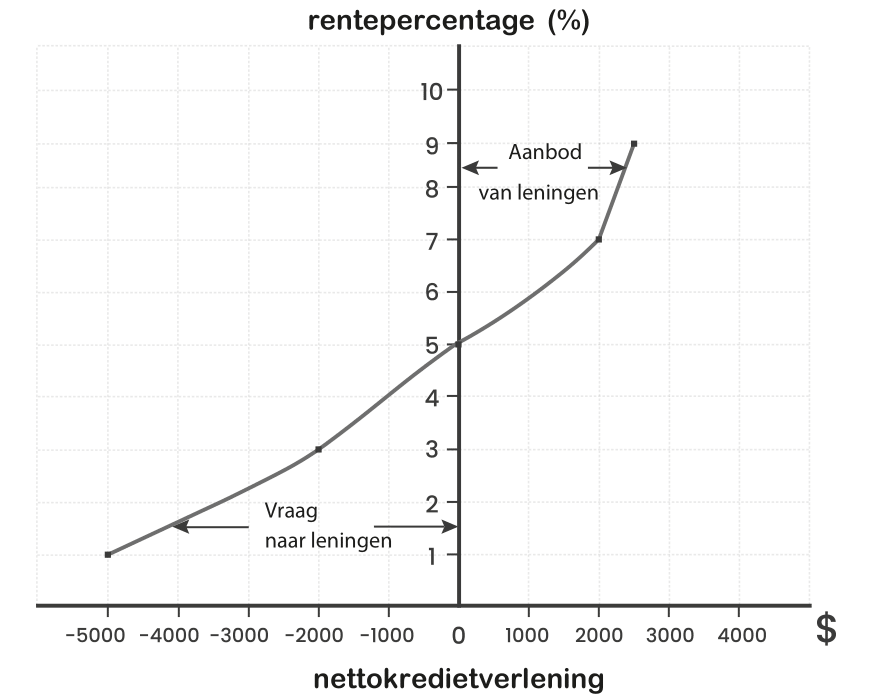
\includegraphics[width=0.9\textwidth]{figures/fig29-1.png}
    \caption[Persoonlijke tijdmarktcurve]{Persoonlijke tijdmarktcurve}
    \label{fig29}
\end{figure}

Op de kapitaalmarkt wordt de som van alle vraag- en aanbodcurven, in feite ieders individuele tijdsvoorkeur\index{tijdsvoorkeur}, samengevoegd tot algemene economische vraag- en aanbodcurven voor uitleenbare middelen. Bij elk gegeven rentetarief is er een totale hoeveelheid kapitaal\index{kapitaal} beschikbaar én gevraagd voor leningen. Aangezien het kapitaal\index{kapitaal} dat beschikbaar is voor leningen toeneemt naarmate de rente\index{rente} stijgt, terwijl het kapitaal\index{kapitaal} dat wordt gevraagd voor leningen afneemt naarmate de rente\index{rente} stijgt, zullen de twee elkaar maar één keer doorkruisen. Dit is het rentetarief dat de kapitaalmarkt in evenwicht brengt. Op dit punt zijn de hoeveelheid leningen perfect gelijk aan de hoeveelheid kapitaal\index{kapitaal} dat is onttrokken aan consumptie\index{consumptie} en beschikbaar is gesteld voor leners.

Het is belangrijk om nogmaals te benadrukken dat tijdsvoorkeur\index{tijdsvoorkeur} en de verdiscontering van de toekomst subjectieve verschijnselen zijn en dat ze niet worden gemeten aan de hand van rentepercentages. Wat er in de hoofden van handelende mensen gebeurt, is het maken van een ordinale rangorde van toekomstige en huidige goederen. Door te worden blootgesteld aan een aanbieding van een rentevoet zijn ze in staat om de impliciete verdiscontering die beschikbaar is op de markt ordinaal te vergelijken met hun persoonlijke verdiscontering en tussen de twee te kiezen. Verder bestaat er niet zoiets als een heersende marktrente. Er zijn alleen individuele rentepercentages die worden beïnvloed door de individuele projecten en de betrokken individuen. De marktrente kan, net als de marktevenwichtsprijs, vooral beschouwd worden als een hulpmiddel om deze economische concepten te begrijpen. Hoewel wiskundige analyse nuttig kan zijn om een begrip van marktverschijnselen over te brengen, is het belangrijk om niet in de val te lopen door ze te behandelen als wetenschappelijke eenheden gebaseerd op nauwkeurige metingen van constanten.

\begin{figure}
\centering
    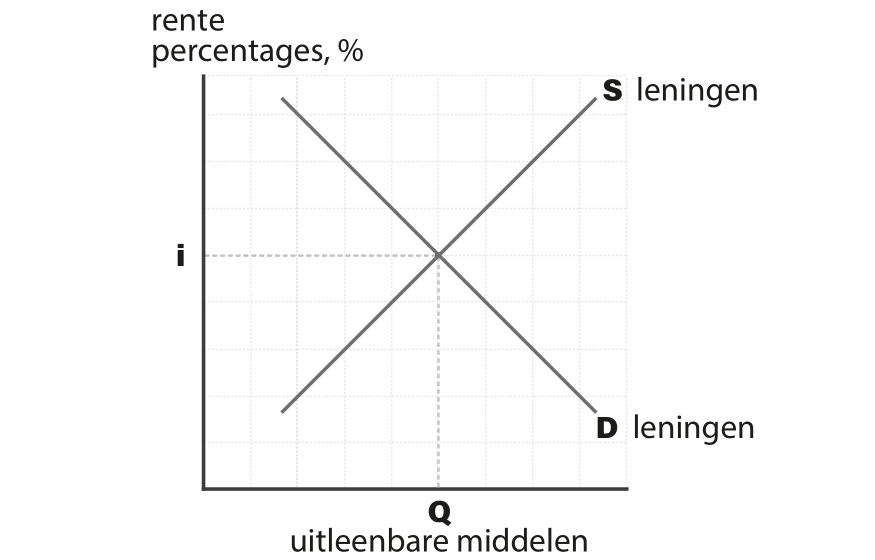
\includegraphics[width=0.7\textwidth]{figures/fig30-1.png}
    \caption[De markt voor leenbaar kapitaal\index{kapitaal}]{De markt voor leenbaar kapitaal\index{kapitaal}}
    \label{fig30}
\end{figure}

Naarmate meer kapitaal\index{kapitaal} wordt ingezet voor economische productie\index{productie}, neemt de productiviteit toe en stijgen de inkomens. Door goed beschermde eigendomsrechten en meer zekerheid over de toekomst zal de tijdsvoorkeur\index{tijdsvoorkeur} naar verwachting verder afnemen, waardoor mensen eerder geneigd zullen zijn om consumptie\index{consumptie} uit te stellen, meer zullen sparen, sneller geld zullen uitlenen en minder snel zelf zullen lenen. De overvloed aan leenbare middelen maakt de financiering mogelijk van een toenemend aantal productieve bedrijven tegen steeds lagere rentetarieven. Als dit proces niet wordt verstoord door oorlog\index{oorlog}, epidemieën, plunderingen, de perverse regeldruk van gecentraliseerde overheden of door met geweld opgedrongen zacht fiatgeld\index{fiatgeld}, zal deze opwaartse trend van toenemend materieel welzijn doorgaan. Dit kan worden beschouwd als het beschavingsproces. Maar hoe ver kan dit proces gaan? Hoe laag kan de rente\index{rente} gaan?

\hypertarget{kan-rente-worden-afgeschaft}{%
\section{Kan rente worden afgeschaft?}\label{kan-rente-worden-afgeschaft}}

Leningen met rente\index{rente} zijn op historisch, politiek en religieus vlak een beladen onderwerp. Veel religies verbieden ze en tot op de dag van vandaag worden ze door veel mensen wereldwijd als immoreel gezien, zelfs in een monetair systeem dat zwaar leunt op kredietcreatie. Mises en de Oostenrijkse economen hebben veel moeite gedaan om uit te leggen dat renteleningen een onlosmakelijk onderdeel van een markteconomie zijn. Ook beargumenteerden ze waarom het een productief element is in de markteconomie. Vanuit het perspectief van de Oostenrijkse economie is rente\index{rente} geen vreemde uitvinding die door leiders aan de maatschappij wordt opgelegd. Zoals alle economische fenomenen vindt rente\index{rente} zijn oorsprong in menselijk handelen\index{menselijk handelen} en in de tijdsvoorkeur\index{tijdsvoorkeur} die in elk individu positief is. Zoals Mises verwoordt:

\begin{blockquotebox}
We kunnen ons nauwelijks een wereld voorstellen waarin natuurlijke rente\index{rente} niet zou bestaan als een onmisbaar element in elke vorm van handelen ... Als er geen natuurlijke rente\index{rente} zou zijn, zouden kapitaalgoederen\index{kapitaalgoederen} niet worden besteed aan onmiddellijke consumptie\index{consumptie} en zou kapitaal\index{kapitaal} niet worden verbruikt. Integendeel, onder zo\textquotesingle n ondenkbare en onvoorstelbare stand van zaken zou er helemaal geen consumptie\index{consumptie} zijn maar alleen sparen, kapitaalopbouw en investeringen. Het is niet de onmogelijke verdwijning van natuurlijke rente\index{rente} die zou leiden tot kapitaalconsumptie, maar het afschaffen van rentebetalingen aan kapitaalbezitters. Juist omdat er natuurlijke rente\index{rente} is en het voldoen aan huidige behoeften de voorkeur heeft boven voldoening op een later tijdstip, zullen de kapitalisten hun kapitaalgoederen\index{kapitaalgoederen} en hun kapitaal\index{kapitaal} consumeren.\footnotemark
\end{blockquotebox}
\footautocite{161}

Pogingen om rente\index{rente} af te schaffen zullen volgens Mises dus niet leiden tot de afschaffing van leningen tegen rente\index{rente} en zullen in plaats daarvan leiden tot de consumptie\index{consumptie} van kapitaalvoorraden omdat, wanneer ze er geen rendement op kunnen maken, spaarders minder gemotiveerd zijn om hun kapitaal\index{kapitaal} te behouden. Mensen verbieden om financiële activa te verhandelen op basis van hun tijdsvoorkeur\index{tijdsvoorkeur} zal hun tijdsvoorkeur\index{tijdsvoorkeur} niet elimineren, het zal altijd hun consumptie\index{consumptie}- en productiebeslissingen blijven beïnvloeden. Als kapitaalbezitters met een positieve tijdsvoorkeur\index{tijdsvoorkeur} geen toegang meer hebben tot de optie om tegen rente\index{rente} te lenen, zullen ze een sterkere prikkel hebben om hun kapitaalvoorraad te consumeren. Het verbieden van rente\index{rente} zorgt er dus voor dat de leners slechter af zijn, aangezien ze geen toegang meer zullen hebben tot broodnodige financiële middelen. Ook de kredietverstrekkers zijn slechter af omdat ze geen rendement meer kunnen halen uit hun spaargeld. Dit schaadt de maatschappij in zijn geheel door de stimulans om te sparen te verminderen, wat leidt tot minder kapitaalopbouw. Een maatschappij zonder rente\index{rente} op leningen is dus minder productief, minder innovatief en minder welvarend.

Vanuit Oostenrijks perspectief is het moeilijk om te beargumenteren dat rente\index{rente} de uitbuiting van de lener is. Er is geen dwang in het leencontract en beide partijen kiezen er vrijwillig voor om het aan te gaan, waardoor er geen wettelijke of morele rechtvaardiging is om het als illegaal te bestempelen, of om als derde partij met geweld te proberen te verhinderen dat de twee partijen transacties met elkaar aangaan.

\begin{blockquotebox}
Er kan daarom geen sprake zijn van het afschaffen van rente\index{rente} door instituten, wetten of bankmanipulatie. Wie rente\index{rente} wil ``afschaffen'' zal de mensen ertoe moeten brengen om een appel die over honderd jaar beschikbaar is niet minder te waarderen dan een appel in het heden. Wat afgeschaft kan worden door wetten en decreten is slechts het recht van de kapitalisten om rente\index{rente} te ontvangen. Zulke decreten zullen echter leiden tot kapitaalconsumptie waardoor de mensheid zeer snel zal terugvallen in de oorspronkelijke staat van natuurlijke armoede.\footnotemark
\end{blockquotebox}
\footautocite{162}

De grootste breuk met de Oostenrijkse orthodoxie in dit boek is het argument waarom de rentevoet in feite kan worden geëlimineerd door een zuiver vrije markt en niet door officiële afschaffing of een decreet. Zoals besproken in het vorige hoofdstuk en in detail uitgelegd door Hoppe in \emph{Democracy}, wordt het beschavingsproces gestart met het verlagen van de tijdsvoorkeur\index{tijdsvoorkeur}, wat resulteert in kapitaalaccumulatie, verhoogde productiviteit en verbeterde levensstandaarden, die op hun beurt verdere daling van de tijdsvoorkeur\index{tijdsvoorkeur} aanmoedigen in een zich voortdurend versterkende spiraal. Oorlogen, ziekten, natuurrampen, toegenomen onzekerheid over de toekomst en groeiende onzekerheid over eigendomsrechten kunnen dit proces tegenhouden door een toename van de tijdsvoorkeur\index{tijdsvoorkeur} te veroorzaken en mensen te dwingen om steeds meer prioriteit te geven aan het heden ten koste van de toekomst.

De historische gegevens ondersteunen deze stelling. Zoals besproken in het vorige hoofdstuk, en zoals gedetailleerd beschreven in de encyclopedische studie over dit onderwerp door Homer en Sylla, heeft de mensheid de afgelopen 5000 jaar een gestage, langdurige daling van de rentetarieven gezien, onderbroken door de eerder genoemde calamiteiten.\autocite{163} Hoppe vat de geschiedenis van de rentedalingen als volgt samen:

\begin{blockquotebox}
    In feite kenmerkt een tendens van dalende rentetarieven de overkoepelende trend van de ontwikkeling van de mensheid. De minimumrente op ``normale veilige leningen'' lag aan het begin van de Griekse financiële geschiedenis in de zesde eeuw voor Christus rond de 16 procent en daalde tot 6 procent tijdens de Hellenistische periode. In Rome daalden ze van meer dan 8 procent tijdens de eerste periode van de Republiek tot 4 procent tijdens de eerste eeuw van het Keizerrijk. In het Europa van de dertiende eeuw was de laagste rente\index{rente} op ``veilige'' leningen 8 procent, waarna ze in de veertiende eeuw daalden tot ongeveer 5 procent. In de vijftiende eeuw daalden ze naar 4 procent, en in de zeventiende eeuw daalden ze naar 3 procent. Aan het einde van de negentiende eeuw waren de minimumrentes verder gedaald tot wel minder dan 2,5 procent.\footnotemark
\end{blockquotebox}
\footautocite{164}

Toch werd deze trend van dalende rentetarieven in de twintigste eeuw tenietgedaan. Waarschijnlijk speelde de transitie naar fiatgeld\index{fiatgeld} een grote rol in deze verschuiving, samen met vele andere factoren die uitvoerig besproken worden in Hoppe\textquotesingle s \emph{Democracy}. Een hypothetisch gedachte-experiment dat hier interessant is, gaat als volgt: wat zou er gebeurd zijn met de rentetarieven als ze in de twintigste eeuw verder waren blijven dalen? Wat zou er zijn gebeurd als de wereld op een goudstandaard\index{goudstandaard} zou zijn gebleven en mensen de mogelijkheid zouden hebben behouden om voor de toekomst te sparen, kapitaal\index{kapitaal} nog overvloediger zou zijn geworden en de productiviteit verder zou zijn toegenomen? Hoe laag zouden de rentetarieven dan zijn geweest?

We kunnen de stelling van Mises dat de natuurlijke rente\index{rente} nooit tot nul kan dalen accepteren, en toch uitkomen op een marktrente van nul. Geld brengt namelijk, net als alle andere goederen, kosten met zich mee, bijvoorbeeld om het simpelweg te bewaren. Welke vorm het ook aanneemt, geld vereist bewaring en opslag, en dit zal altijd kosten met zich meebrengen die niet nul zijn en er zal altijd een risico\index{risico} van diefstal, verlies of schade aan vast hangen. Deze kosten kunnen op verschillende manieren worden betaald, zoals via de aankoop van een kluis of een opslagplaats, door de kosten van een depositorekening bij een bank\index{bank} of door het bedrag te verzekeren. Of er kan betaald worden in de vorm van diefstal en verlies, wat een risico\index{risico} is dat altijd bestaat. Er moeten bepaalde kosten, die niet nul zijn, worden betaald om geld te bewaren. De opportuniteitskosten van het uitlenen liggen voor de geldschieter niet in het volledig behouden van hun nominale rijkdom, maar niet uitlenen zal voor hem betekenen dat de waarde van het geld langzaam daalt door de kosten om het veilig te houden.

Als de tijdsvoorkeur\index{tijdsvoorkeur} samen met de natuurlijke rente\index{rente} blijft dalen, kan de marktrente uiteindelijk lager worden dan de bewaarkosten van het geld. In zo'n situatie zou de geldschieter graag geld uitlenen tegen een nominale rente\index{rente} van 0\%, omdat dit een beter rendement is dan het geld gewoon aan te houden, wat een negatief rendement zou betekenen. In plaats van rente\index{rente} per decreet af te schaffen, zou het voortdurende proces van beschaving\index{beschaving}, kapitaalaccumulatie en de daling van tijdsvoorkeur\index{tijdsvoorkeur} het lenen met rente\index{rente} op natuurlijke wijze volledig kunnen elimineren.

Een daling van de tijdsvoorkeur\index{tijdsvoorkeur} vergroot de overvloed aan kapitaal\index{kapitaal} en naarmate deze overvloed verder toeneemt, zal de prijs\index{prijs} van kapitaal\index{kapitaal}, in de vorm van rente\index{rente}, dalen. Een beschaving\index{beschaving} die voortdurend vooruitgang boekt, ervaart een daling van haar tijdsvoorkeur\index{tijdsvoorkeur}, wat leidt tot meer toekomstige voorzieningen en een groter moreel plichtsbesef met betrekking tot toekomstige generaties. Dit resulteert in een grote overvloed aan kapitaal\index{kapitaal}. Wanneer mensen in het bezit zijn van grotere hoeveelheden kapitaal\index{kapitaal}, neemt ook de vraag naar leningen af. Op dat moment kan een lener zich verzekeren van een lening\index{lening} van de vele beschikbare kredietverstrekkers door simpelweg te beloven om het geld volledig terug te betalen. Dit bespaart de kredietverstrekker namelijk de kosten van opslag en verzekering, of het risico\index{risico} op diefstal en verlies.

Naarmate de rente\index{rente} samen met de tijdsvoorkeur\index{tijdsvoorkeur} daalt, wordt de asymmetrie van de leenovereenkomst steeds onaantrekkelijker voor de kredietverstrekker. Waarom het risico\index{risico} nemen om al het kapitaal\index{kapitaal} te verliezen in ruil\index{ruil} voor zo\textquotesingle n mager rendement? Het leencontract beperkt het opwaartse voordeel voor de kredietverstrekker, maar er is geen enkele garantie dat de kredietverstrekker zijn geld echt terugkrijgt. Risico bestaat, en het risico\index{risico} van een volledig en catastrofaal verlies kan nooit volledig worden weggenomen. In het moderne, op fiat\index{fiat} gebaseerde economische systeem, is het faillissementsrisico van banken sterk verminderd door het risico\index{risico} over te dragen naar de nationale valuta zelf. Leningen worden in feite gegarandeerd door de mogelijkheid van de centrale bank\index{centrale bank} om de kredietverstrekkers schadeloos te stellen bij eventuele wanbetalingen op hun portfolio. Dit is de reden waarom de FDIC (Federal Deposit Insurance Corporation) in staat is om bankrekeningen in de moderne wereld te garanderen, maar in de hypothetische samenleving van dit scenario is dit niet iets waarvan je zou verwachten dat het bestaat. Kapitaalaccumulatie en een daling van de tijdsvoorkeur\index{tijdsvoorkeur} zouden niet vergevorderd kunnen zijn in een samenleving met inflatoir fiatgeld\index{fiatgeld} dat door de centrale bank\index{centrale bank} gebruikt kan worden om banken te redden, omdat dergelijk geld het sparen zou ontmoedigen en het niet zou toelaten dat de tijdsvoorkeur\index{tijdsvoorkeur} en rentetarieven dalen. We zouden zo\textquotesingle n punt alleen kunnen bereiken met een harde geldstandaard die sparen aanmoedigt en die banksteun of faillissementsbescherming voor kredietverstrekkers uitsluit. In zo\textquotesingle n wereld van lage tijdsvoorkeur\index{lage tijdsvoorkeur}, hard geld\index{hard geld} en zonder financiële reddingsoperaties wordt lenen tegen rente\index{rente} onwaarschijnlijk. Kredietverstrekkers zouden een zeer klein rendement behalen, terwijl het volledige bedrag in rook op kan gaan. Als ze het volledige risico\index{risico} op zich nemen, zouden ze liever ook meegenieten van de winsten via een investering in aandelen.

In een wereld van grote overvloed aan kapitaal\index{kapitaal}, verwaarloosbaar lage rentes, of zelfs rentetarieven van nul procent, zullen mensen die kredietwaardig zijn geen probleem hebben om kapitaal\index{kapitaal} van vrienden en familie te lenen in geval van nooduitgaven of tegenspoed. Uitlenen zonder rente\index{rente} bespaart de eigenaar van het geld de noodzaak om geld uit te geven aan opslag en verlost hem van het risico\index{risico} van verlies. Bij een zeer lage tijdsvoorkeur\index{lage tijdsvoorkeur} is uitlenen aan een vertrouwde lener dus voordeliger dan het geld zelf aanhouden. Voor zakelijke investeringen is het echter waarschijnlijker dat de markt zich voornamelijk zal richten op aandelen. In een dergelijke wereld zal het bankwezen netjes worden opgedeeld in twee categorieën: investeringsbanken en depositobanken.

De hierboven besproken gouden regel van Mises stelt dat goederenkrediet volledig moet worden gedekt door spaargeld met dezelfde looptijd van de lening\index{lening}. Maar zonder een mogelijke ultieme geldschieter (of: \emph{lender of last resort}) en bij een nominale rente\index{rente} van nul, zal deze regel een extra bepaling krijgen: de kredietverlener krijgt een vooraf overeengekomen aandeel in de winst van de onderneming. Met andere woorden, er zal geen kredietverstrekker zijn, maar een investeerder met eigen vermogen in de onderneming.

Inzicht in de tijdsvoorkeurtheorie van rentetarieven vanuit het Oostenrijkse perspectief, ook wel bekend als de agiotheorie, kan helpen om de historische en religieuze argumenten tegen rente\index{rente} te verklaren. In een wereld waarin de nominale rentevoet nul is, is de tijdsvoorkeur\index{tijdsvoorkeur} zo laag dat de natuurlijke rente\index{rente} lager is dan de bewaarkosten van geld. Religieuze mandaten tegen rente\index{rente} kunnen worden beschouwd als instructies voor de religieuzen om hun tijdsvoorkeur\index{tijdsvoorkeur} te verlagen tot het punt waarop het lenen met rente\index{rente} voor hen niet meer aantrekkelijk is. Geloof in het hiernamaals kan mogelijk bevorderlijk werken voor het verlagen van de tijdsvoorkeur\index{tijdsvoorkeur}. Verwachtingen om tot in de eeuwigheid te leven, en dus oneindig veel beloningen en straffen voor hun daden te ervaren, zouden kunnen leiden tot een oneindig lage afwaardering van toekomstige gevolgen.

Terwijl religies en tradities deze realiteit aan hun gelovigen proberen op te leggen door middel van leefregels, is de moderne markteconomie het instrument dat ons in de praktijk naar deze realiteit stuurt, allemaal door middel van constante kapitaalaccumulatie, arbeidsdeling\index{arbeidsdeling}, technologische vooruitgang en het verlagen van tijdsvoorkeur\index{tijdsvoorkeur}. Met andere woorden, als de processen van de markt en de beschaving\index{beschaving} ononderbroken doorgaan, neemt het verdisconteren van de toekomst af tot het punt waarop rente\index{rente} wordt geëlimineerd. Dit resulteert in een systeem zonder woekerrente, vergelijkbaar met het traditionele christelijke en islamitische bankieren.

Joseph Schumpeter geeft een goede samenvatting van het werk van Eugene Böhm-Bawerk, de Oostenrijkse econoom die het meest bijdroeg aan de ontwikkeling van de Oostenrijkse rentetheorie.

\begin{blockquotebox}
    {[}Rente{]} is als het ware de rem of de regelaar die individuen ervan weerhoudt de economisch\index{economisch} toelaatbare verlenging van de productieperiode te overschrijden en die voorzieningen voor huidige behoeften afdwingt -- wat in feite hun urgentie onder de aandacht van ondernemers brengt. Het weerspiegelt daardoor de relatieve intensiteit waarmee in elke economie toekomstige en huidige belangen zich doen gelden, en dus ook de intelligentie en de morele kracht van een volk -- hoe hoger deze zijn, hoe lager de rentevoet zal zijn. Daarom weerspiegelt de rentevoet het culturele niveau van een natie; want hoe hoger dit niveau, hoe groter de beschikbare voorraad consumptiegoederen\index{consumptiegoed}, hoe langer de productieperiode, hoe kleiner, volgens de wet van de afnemende opbrengst, de meeropbrengst die verdere verlenging van de productieperiode zou opleveren, en dus hoe lager de rentevoet. En hier hebben we Böhm-Bawerk\textquotesingle s wet van de dalende rente\index{rente}, zijn oplossing voor dit oude probleem waarover de slimste koppen van onze wetenschap zonder succes het hoofd hebben gebroken.\footnotemark
\end{blockquotebox}
\footautocite{165}

Of een voortdurende daling van de tijdsvoorkeur\index{tijdsvoorkeur} de rentetarieven echt zal doen dalen tot een nominaal nultarief is een vraag die losstaat van de economische doeltreffendheid van een dwingend verbod op rente\index{rente}. Zonder de vereiste lage tijdsvoorkeur\index{lage tijdsvoorkeur} zal het verbieden van renteleningen waarschijnlijk leiden tot meer consumptie\index{consumptie}, minder sparen en uitlenen, en waarschijnlijk minder investeringen in het algemeen. Het is mogelijk dat lenen tegen rentes het enige is dat de rentelening kan laten verdwijnen. Door sparen te stimuleren en kapitaalaccumulatie te vergroten, leidt de rentelening tot een daling van de tijdsvoorkeur\index{tijdsvoorkeur} en rentetarieven, tot ze uiteindelijk compleet verdwijnen.
